\begin{questions}

\question{
Simulate nonlinear diffusion using TRBDF2.c.  Plot (in one figure)
$u(x, t)$ for $t$ = 0, 500, 1000, 1500, 2000 sec ($t_{comp}$ = 0, 0.5,
1, 1.5, 2) using the following parameters (for $t$ = 1000 sec):

\begin{verbatim}
Enter the max value of t in 1000 sec: 1
Enter the max number of timesteps: 100000
Enter initial FACTOR & MAX_FACTOR for dt = FACTOR * dt_euler(t = 0): 10 100  
Enter MIN_FACTOR for dt (e.g. 0.01): 0.01
Enter the min & max values of x in 0.1 microns: 0 10
Enter the number of dx: 100
\end{verbatim}
}
\begin{solution}
\begin{figure}[H]
\centering     %%% not \center
{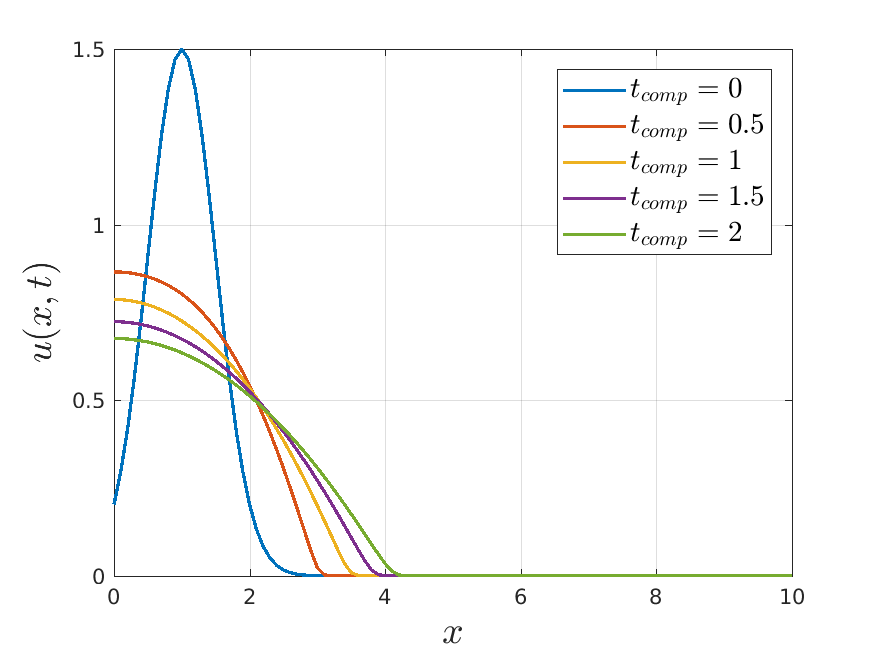
\includegraphics[scale=0.7]{problem4.png}}
\caption{Funcion $u(x,t)$ for different values of time.}
\end{figure}
\end{solution}
\end{questions}
